\section{Results and analysis}
\label{sec:analysis}

\subsection{Property distributions}
Here we will look at the frequency distributions (histograms) comparing the characteristics of CPSBs, RPSBs an their control galaxies.

TODO: include a definition of the S\'ersic index \citep{1963BAAA....6...41S,sérsic1968atlas}, its significance in this context: ellipticals vs. disks, and how it is measured. The surface brightness profile of a galaxy is generally a function of radius from the nucleus. The rate of change of brightness can be described by the S\'ersic function. Low values of SI ~1 relate to disc-like spiral galaxies, whereas higher SI values of 3 or more are measured in galaxies with compact bright nuclei, indicative of more evolved systems.  

We compare the distributions of CPSBs with that of the RPSB sample in terms of S\'ersic index, stellar mass, and redshift. These distributions are taken from the data in Tables \ref{tab:my-CPSBs} and \ref{tab:my-RPSBs}. The frequency distribution histograms are plotted in Figures \ref{fig:Sersic-plot}, \ref{fig:stellar-mass-plot} and \ref{fig:redshift-plot} respectively.

\begin{figure}
    \centering
    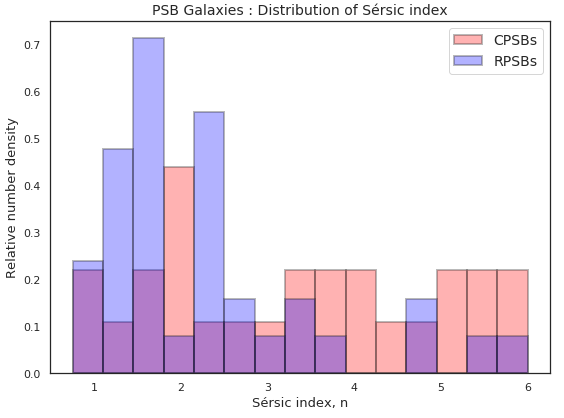
\includegraphics[width=\columnwidth]{images/JupyterPlots/Dist-Sersic-Index-All.png}
    \caption{Distribution of S\'ersic index (SI) values. The relative number density distribution of the S\'ersic index value for 26 CPSBs (red histogram) and 36 RPSBs (blue) are plotted. Those PSB galaxies with unreliable SI values (5) have been excluded. Generally CPSBs show higher SI values than RPBs. This indicates that CPBs tend to have concentrated nuclei contrary to the more disc-like RPSBs.}
    \label{fig:Sersic-plot}
\end{figure}

\begin{figure}
    \centering
    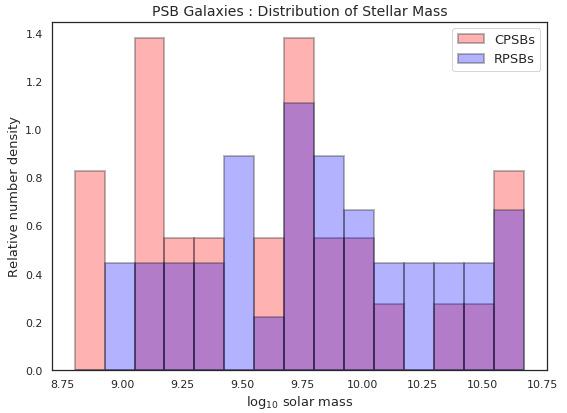
\includegraphics[width=\columnwidth]{images/JupyterPlots/Dist-Stellar-Mass-All.png}
    \caption{Distribution of Stellar mass of our sample of CPSBs (rad) and RPSBs (blue). On the scale of $\log_{10}$\Msun\ a fairly uniform distribution of stellar mass is apparent for both populations, CPSBs and RPSBs.}
    \label{fig:stellar-mass-plot}
\end{figure}

\begin{figure}
    \centering
    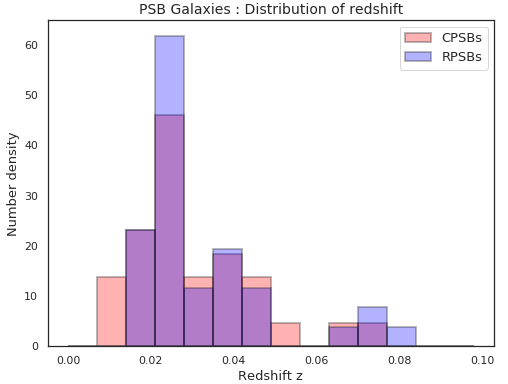
\includegraphics[width=\columnwidth]{images/JupyterPlots/Dist-z-All.png}
    \caption[PSB distribution in redshift]{Distribution in redshift. The redshift distribution of the CPSB sample (shaded in red) is similar to that of the RPSB sample (blue).}
    \label{fig:redshift-plot}
\end{figure}

\begin{figure}
    \centering
    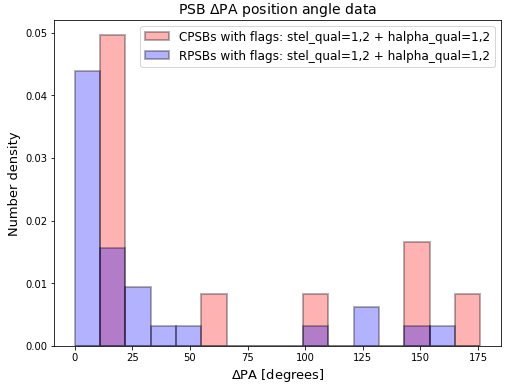
\includegraphics[width=\columnwidth]{images/JupyterPlots/Dist-Delta-PA-All-GoodFlags.png}
    \caption[Distribution of PSB velocity field position angles]{Distribution of PSB galaxy velocity map position angles for those PSBs with stellar velocity and gas velocity characteristics flagged as 'good' as denoted in the legend (details are provided in the text). CPSB PA density weights are plotted in red, RPSB PA weights in blue.}
    \label{fig:deltaPAdistribution}
\end{figure}

The velocity field position angle variance of the CPSB and PSB control galaxies is shown in Figure \ref{fig:controlDeltaPAs}. Both sets of control galaxies have low values of velocity field $\Delta$PAs, i.e. the stellar velocity and gas velocity fields are generally aligned.

\begin{figure}
    \centering
    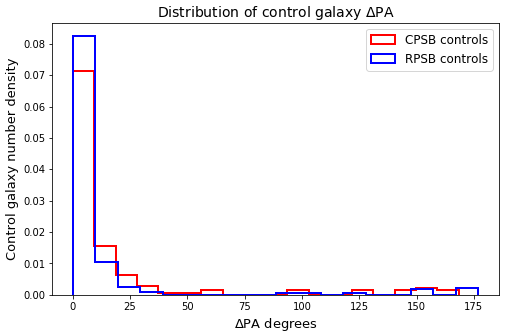
\includegraphics[width=\columnwidth]{images/JupyterPlots/Distribution-of-control-galaxy-deltaPA.png}
    \caption[Distribution of control galaxy $\Delta$PAs]{Distribution of control galaxy stellar and gas velocity field $\Delta$PAs.}
    \label{fig:controlDeltaPAs}
\end{figure}

\begin{figure}
    \centering
    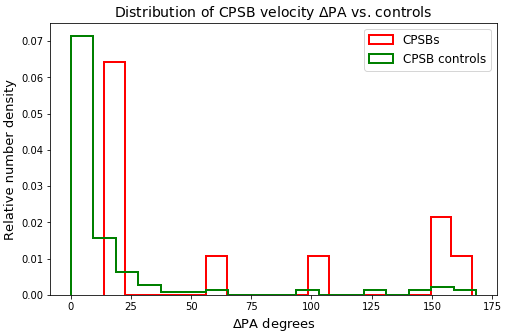
\includegraphics[width=\columnwidth]{images/JupyterPlots/Distribution-of-CPSB-dPA-vs-controls.png}
    \caption{Distribution of CPSB stellar-gas velocity $\Delta$PA vs. controls.}
    \label{fig:CPSBvsControlDeltaPAs}
\end{figure}

\begin{figure}
    \centering
    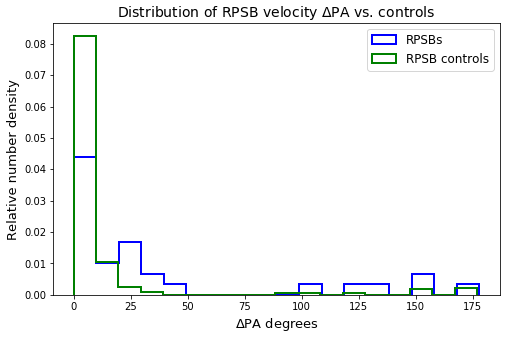
\includegraphics[width=\columnwidth]{images/JupyterPlots/Distribution-of-RPSB-dPA-vs-controls.png}
    \caption{Distribution of RPSB stellar-gas velocity $\Delta$PA vs. controls.}
    \label{fig:RPSBvsControlDeltaPAs}
\end{figure}

\subsection{The KS-test}
The Kolmogorov-Smirnov test: a statistical test to determine if two samples come from the same underlying distribution, see e.g. \citet{hodges1958significance}. We implement this test using the SciPy package \texttt{scipy.stats.kstest} module\footnote{\href{}{https://docs.scipy.org/doc/scipy/reference/generated/scipy.stats.ks\_2samp.html}}.

We ran the two-sided K-S test statistic on the distribution of $\Delta$ position angles obtained from the \texttt{kinemetry} analysis. The results are given in Table \ref{tab:K-S-tests}. The statistical significance inferred from the from the K-S test is that a high value of the test statistic, typically > 0.1, together with a low p-value, < 0.1 [TODO: validate these values] indicates that the samples are drawn from different statistical distributions. Here we note that the CPSB and RPSB samples originate from different distributions, and also each sample is from a different distribution from its corresponding control galaxy sample. The Python implementation \texttt{scipy.stats.ks\_2samp} accepts samples of different sizes.

\begin{table}
\caption[Kolmogorov-Smirnov statistical test]{Kolmogorov-Smirnov statistical test on various $\Delta$PA sample distributions. A high value of the K-S statistic > 10\%, together with a low p-value, < 10\% indicates that the samples come from different statistical distributions.}
\label{tab:K-S-tests}
\begin{tabular}{llcc}
\hline
$\Delta$PA sample 1  & $\Delta$PA sample 2 & K-S statistic & p-value \\
\hline
CPSB & RPSB & 0.467 & 0.040 \\
CPSB & CPSB controls & 0.755 & 0.000 \\
RPSB & RPSB controls & 0.520 & 0.000 \\
CPSB controls & RPSB controls & 0.197 & 0.001 \\
\hline
\end{tabular}
\end{table}
